% Author: Kimberly Golubeva
% Date: 21 August 2020
% Lauren DeDieu, Jerrod M.~Smith, Kimberly Golubeva and Christian Bagshaw
% A Resource Bank for Writing Intensive Mathematics Courses
% This work is licensed under a  Creative Commons Attribution-NonCommercial-ShareAlike 4.0 International License
% http://creativecommons.org/licenses/by-nc-sa/4.0/
\section{Cartesian Product Set Equality}

\begin{xca}{xca:cart_product}
Prove or disprove the following statement. For all sets $A,B$ and $C$, if $A \times B = A \times C,$ then $B=C.$ 
\end{xca}

\begin{flaw}{flaw:cart_product} %change the label
Yes, this statement is true. By considering the picture below,
\center{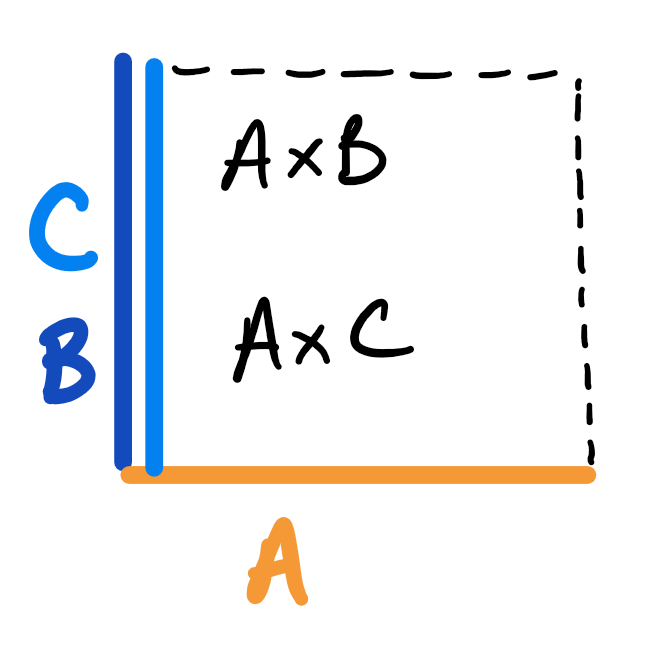
\includegraphics{Discrete/cart_product.PNG}}

we see that if the area of $A \times B$ equals the area of $A \times C$, then it must be the case that $B=C.$

\end{flaw}

\clearpage
\subsection{Error classification}

%Provide a brief classification and explanation of the errors in the Flawed Proof \ref{flaw:proof1}. %change the label

There are several errors
% is only one error ... etc.
 in the Flawed Proof \ref{flaw:cart_product}. %change the label

 
 \begin{description}
 	\item[F-Eg:] Proof by picture/example.
 	\item[C-FS:] The statement in question is false.
 	\item[F-EO-FS:] False statement caused omission of majority of the proof (i.e. a counterexample).
 \end{description}

 
\subsubsection{Error codes}
\begin{itemize}
	\item 	Fundamental Proof by Example (F-Eg)
	\item   Content False Statement (C-FS)
	\item   Fundamental Error-caused Omission resulting from False Statement (F-EO-FS)
\end{itemize}
See Section \ref{sec-error} for more information about error classifications.

\clearpage
\subsection{Corrected proof}

The following is a corrected version of Flawed Proof \ref{flaw:cart_product}. %change the label

\begin{prf}{prf:cart_product} %change the label
This statement is false. Consider the following counterexample. Let $A = \varnothing, B = \{1\}$ and $C=\{1,2\}.$ Then $A \times B = \varnothing$ and $A \times C = \varnothing,$ but $B \neq C$ since $2 \in C$  and $2 \notin B.$
\end{prf}